\begin{frame}[allowframebreaks]
  \frametitle{A New Perspective}
  $$S:y^2 = 2s^4 + 8ms^2 + 16m^2 + 16m$$
  \phantom{hi}
  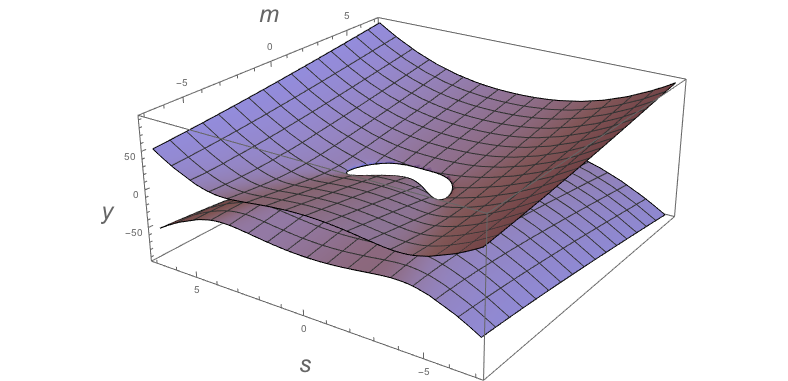
\includegraphics[width=\textwidth]{SPlot.png}
  
\framebreak
  
  So far,
	$$S:y^2 = 2s^4 + 8ms^2 + 16m^2 + 16m$$
	\phantom{hi}
	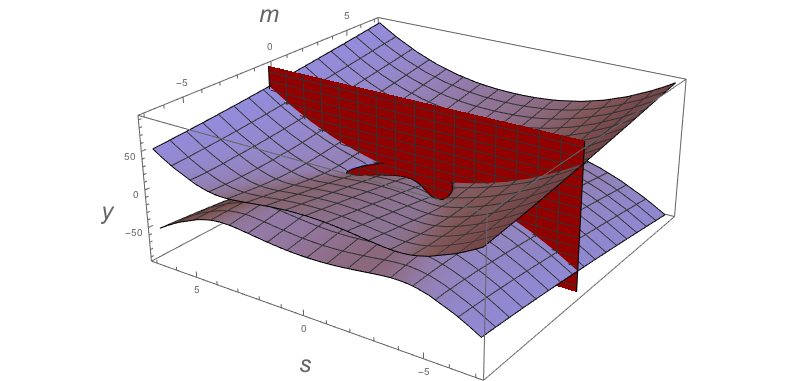
\includegraphics[width=\textwidth]{ECPlot.png}

\framebreak

	$$S:y^2 = 16m^2 + (16+8s^2)m + 2s^4$$
	\phantom{hi}
	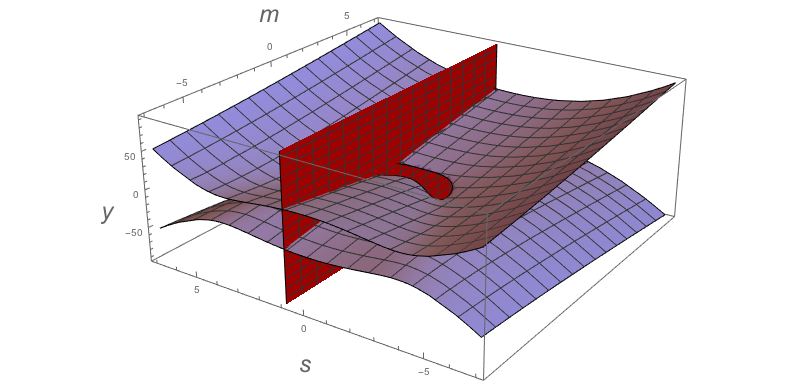
\includegraphics[width=\textwidth]{CSPlot.png}
	
	\framebreak
	
	This is a conic! $$y^2 = am^2 + bm + c$$
	\phantom{hi}
	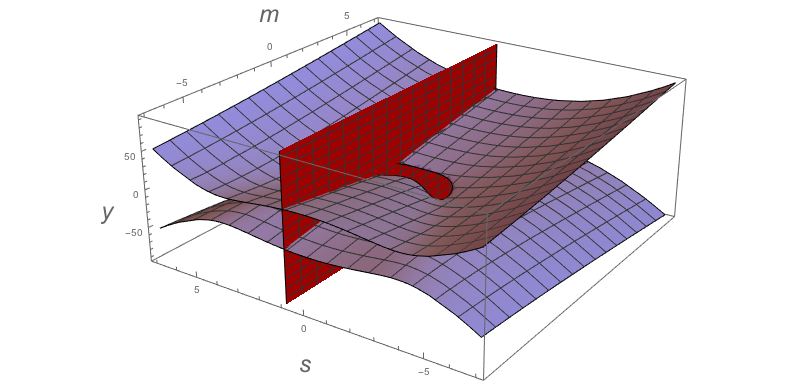
\includegraphics[width=\textwidth]{CSPlot.png}
\end{frame}

\begin{frame}
	\frametitle{Rational Projection}
	For any $s$, we have
	$$y^2 = 16m^2 + (16+8s^2)m + 2s^4.$$
	\pause
	To use projection, we need a point on this curve.\\
	\pause
	Luckily, we can use the point at infinity!
\end{frame}
	
\begin{frame}
	\frametitle{Rational Projection}
	$$S: y^2 = 16m^2 + (16+8s^2)m + 2s^4$$
	\pause
	\begin{obs}
		We're only looking for \textbf{rational} solutions.
	\end{obs}
	\pause
	$$\mbox{Let }y = \frac{Y}{Z}\mbox{ and }m = \frac{M}{Z}.$$
	\pause
	\begin{defn}
		The \textbf{homogeneous form} of $S$ is
		$$S: Y^2 = 16 M^2 + (8 s^2 + 16) M Z + 2 s^4 Z^2.$$
	\end{defn}
\end{frame}

\begin{frame}
	\frametitle{Rational Projection}
	If $Z=0$...
	\pause
	$$Y^2 = 16 M^2 + (8 s^2 + 16) M Z + 2 s^4 Z^2$$
	\pause
	$$Y^2 = 16 M^2 +\text{ \hcancel{\ensuremath{(8 s^2 + 16) M Z}}} + \text{ \hcancel{\ensuremath{2 s^4 Z^2}}}$$
	\pause
	$$ Y^2 = 16 M^2 $$
	\pause
	$$ Y=\pm 4 M$$
\end{frame}

\begin{frame}
	\frametitle{Rational Projection}
	\begin{obs}
		The point $[M:Y:Z]=[1:4:0]$ is a solution to the homogeneous form of $S$.
	\end{obs}
	\pause
	\begin{center}
		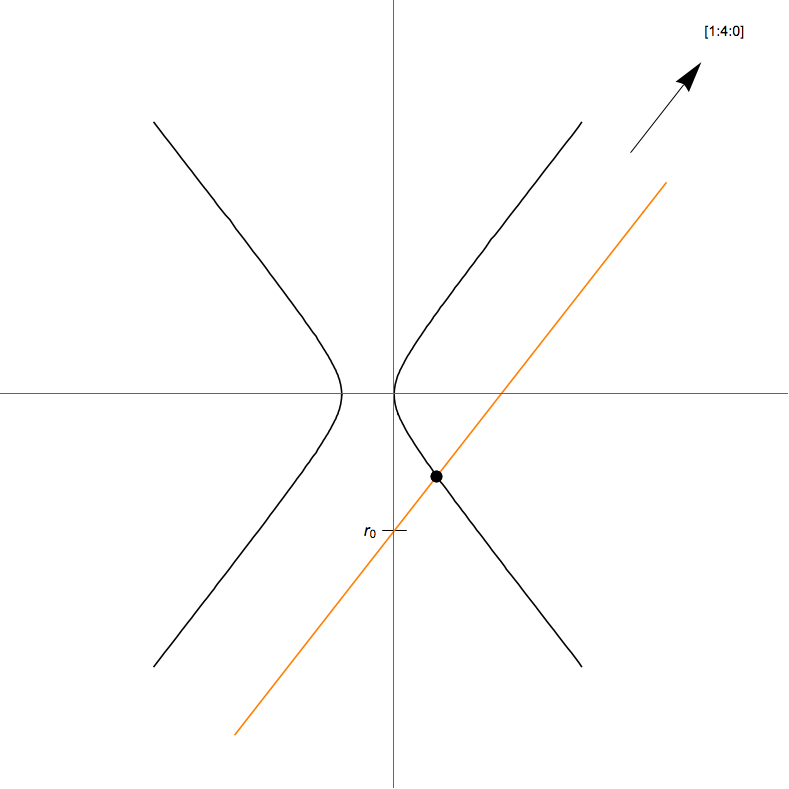
\includegraphics[width=.5\textwidth]{projection-from-infinity.png}
	\end{center}
\end{frame}



























